\documentclass{article}
%% Useful packages
\usepackage[utf8]{inputenc}
\usepackage[a4paper,left=2cm,right=2cm,top=2cm,bottom=2cm]{geometry}
\usepackage{crop,graphicx,amsmath,array,color,amssymb,fancyhdr,lineno}
\usepackage{flushend,stfloats,amsthm,chngpage,times,,lipsum,lastpage} 
\usepackage{calc,listings,color,wrapfig,tabularx,longtable,enumitem}
\usepackage[style=numeric-comp,backend=biber]{biblatex}
\addbibresource{Refs.bib}
\usepackage{lineno}
%%%%%%%%%%%%   Header and Footer  %%%%%%%%%%%%%
\pagestyle{fancy}
\fancypagestyle{plain}{%
  \renewcommand{\headrulewidth}{0pt}%
  \fancyhf{}%
}

\title{%
  First Assignment \\
  \large Equivalent representations of orientation matrices}
\author{Surname Name}

\begin{document}
\begin{titlepage}

\newcommand{\HRule}{\rule{\linewidth}{0.5mm}} % Defines a new command for the horizontal lines, change thickness here

%----------------------------------------------------------------------------------------
%	LOGO SECTION
%----------------------------------------------------------------------------------------
\center

\includegraphics[width=5cm]{Title/Unige-logo.jpeg}\\[1cm] % Include a department/university logo - this will require the graphicx package
 
%----------------------------------------------------------------------------------------

\center % Center everything on the page

%----------------------------------------------------------------------------------------
%	HEADING SECTIONS
%----------------------------------------------------------------------------------------

\textsc{\Huge Università degli studi di Genova}\\[1cm] % Name of your university/college
\textsc{\LARGE DIBRIS}\\[0.3cm]
\textsc{\Small Department of Computer Science and Technology,}\\
\textsc{\Small Bioengineering, Robotics and System Engineering}\\[1cm] % Minor heading such as course title
\textsc{\LARGE{Modelling and Control of Manipulators}}\\[1cm] % Major heading such as course name

%----------------------------------------------------------------------------------------
%	TITLE SECTION
%----------------------------------------------------------------------------------------
\makeatletter
\HRule \\[0.4cm]
{ \huge \bfseries Second Assignment}\\[0.2cm] 
{\Large \bfseries Manipulator Geometry and Direct Kinematics}\\
% Title of your document
\HRule \\[1.5cm]
 
%----------------------------------------------------------------------------------------
%	AUTHOR SECTION
%----------------------------------------------------------------------------------------

\begin{minipage}{0.4\textwidth}
\begin{flushleft} \large
\emph{Author:}\\[0.2cm]
Surname Name % Your name
\\[1.2em]
\emph{Student ID:}\\[0.2cm]
s0000000 \\[1.2em]
\end{flushleft}
\end{minipage}
~
\begin{minipage}{0.4\textwidth}
\begin{flushright} \large
\emph{Professors:} \\[0.2cm]
Enrico Simetti\\
Giorgio Cannata  \\[1.2em] % Supervisor's Name

\emph{Tutors:} \\[0.2cm]
Andrea Tiranti\\
Luca Tarasi\\
George Kurshakov
% second marker's name
\end{flushright}
\end{minipage}\\[2cm]
\makeatother

% If you don't want a supervisor, uncomment the two lines below and remove the section above
%\Large \emph{Author:}\\
%John \textsc{Smith}\\[3cm] % Your name

%----------------------------------------------------------------------------------------
%	DATE SECTION
%----------------------------------------------------------------------------------------

{\large \today}\\[2cm] % Date, change the \today to a set date if you want to be precise

\vfill % Fill the rest of the page with whitespace

\end{titlepage}

\sffamily

\fancyhf{}
\fancyhead[L]{Surname Name - s0000000}
\fancyhead[R]{Modelling and Control of Manipulators - Assignment 1}
\fancyfoot[R]{ \bf\thepage\ \rm }%

\newpage
\tableofcontents

\section*{}
\begin{longtable}{|p{4cm}|p{4cm}|p{4cm}|}
    \hline
    Mathematical expression & Definition & MATLAB expression \\
    \hline 
    $<w>$ & World Coordinate Frame &  w\\[0.4cm]
    $^a_b R$ & Rotation matrix of frame $<b>$ with respect to frame $<a>$  & aRb \\[1.2cm]
    $^a_b T$ & Transformation matrix of frame $<b>$ with respect to frame $<a>$ & aTb \\
    $^a O_b$ & Vector defining frame $<b>$ wit respect to frame $<a>$ & aOb\\
    [1.2cm]
    \hline
    \caption{Nomenclature Table}
\end{longtable}

\section{Assignment description}
The first assignment of Modelling and Control of Manipulators focuses on the geometric fundamentals and algorithmic tools underlying any robotics application. The concepts of transformation matrix, orientation matrix and the equivalent representations of orientation matrices (Equivalent angle-axis representation and Euler Angles) will be reviewed.

The first assignment is \textbf{mandatory} and consists of 5 different exercises. You are asked to:
\begin{itemize}
    \item Download the .zip file called MCM-LAB1 from the Aulaweb page of this course.
    \item Implement the code to solve the exercises on MATLAB by filling the predefined files called "\textit{main.m}", "\textit{AngleAxisToRot.m}", "\textit{RotToAngleAxis.m}", "\textit{YPRToRot.m}" and "\textit{RotToYPR.m}".
    \item Write a report motivating the answers for each exercise, following the predefind format on this document.
\end{itemize}

\subsection{Exercise 1 - Angle-Axis to Rotation Matrix}
A particularly interesting minimal representation of 3D rotation matrices is the so-called angle-axis representation, where a rotation is represent by the axis of rotation \begin{math}\textbf{h}\end{math} and the angle $\theta$. Any rotation matrix can be represented by its equivalent angle-axis representation by applying the Rodrigues Formula.

%\[ R(^* \textbf{v},\theta) = e^{[^*\textbf{v}\times]\theta} = e^{[\rho\times]} =  \textbf{I}_{3x3} + [^* \textbf{v}\times] \sin(\theta) + [^* \textbf{v}\times]^2 (1-\cos(\theta))\]


\textbf{Q1.1} Given an angle-axis pair \begin{math}(\textbf{h},\theta)\end{math}, implement on MATLAB the Rodrigues formula, computing the equivalent rotation matrix, \textbf{WITHOUT} using built-in matlab functions. The function signature will be


\begin{center}\textit{function R = AngleAxisToRot(h,theta)}\end{center}


Then test it for the following cases and briefly comment the results obtained:
\begin{itemize}
    \item \textbf{Q1.2}\hspace{10mm} \begin{math} \textbf{h} = [1,0,0]^T\end{math} and  \begin{math} \theta = 90^\circ \end{math}
    \item \textbf{Q1.3}\hspace{10mm} \begin{math} \textbf{h} = [0,0,1]^T\end{math} and  \begin{math} \theta = \pi/3 \end{math}
    \item \textbf{Q1.4}\hspace{10mm} \begin{math} \mathbf{\rho} = [-\pi/3, -\pi/6 ,\pi/3];\end{math}
\end{itemize}
\textbf{Note that $\mathbf{\rho} = \textbf{h}\theta$}.
%\subsection{Exercise 2 - Inverse Equivalent Angle-Axis Problem}
\subsection{Exercise 2 - Rotation Matrix to Angle-Axis}
Given a rotation matrix \begin{math}R\end{math}, the problem of finding the corresponding angle-axis representation \begin{math}(\textbf{h},\theta)\end{math} is called the Inverse Equivalent Angle-Axis Problem.
\newline


\textbf{Q2.1} Given a rotation matrix \begin{math}R\end{math}, implement on MATLAB the Equivalent Angle-Axis equations \textbf{WITHOUT} using built-in matlab functions. The function signature will be


\begin{center}\textit{function [h,theta] = RotToAngleAxis(R)}\end{center}


You \textbf{MUST} check that the input is a valid rotation matrix. Test it for the following cases and briefly comment the results obtained:

\begin{itemize}
    \item \textbf{Q2.2}\hspace{10mm} $R = \begin{pmatrix}
        1 & 0 & 0 \\
        0 & 0 & -1 \\
        0 & 1 & 0
    \end{pmatrix}$
    
    \item \textbf{Q2.3}\hspace{10mm} $R = \begin{pmatrix}
        1& -\sqrt{3}/2 & 0 \\
        \sqrt{3}/2 & 0.5 & 0 \\
        0 & 0 & 1
    \end{pmatrix}$
    
    \item \textbf{Q2.4}\hspace{10mm} $R = \begin{pmatrix}
        1 & 0 & 0 \\
        0 & 1 & 0 \\
        0 & 0 & 1
    \end{pmatrix}$
    
    \item \textbf{Q2.5}\hspace{10mm} $R = \begin{pmatrix}
        -1 & 0 & 0 \\
        0 & -1 & 0 \\
        0 & 0 & 1
    \end{pmatrix}$
\end{itemize}

\subsection{Exercise 3 - Euler Angles to Rotation Matrix}
Any orientation matrix can be expressed in terms of three elementary rotations in sequence. Consider the Yaw Pitch Roll (YPR) representation, where the sequence of the rotation axes is Z-Y-X.
\newline

\textbf{Q3.1} Given a triplet of YPR angles ($\psi$, $\theta$, $\phi$), compute the equivalent rotation matrix representation \textbf{WITHOUT} using built-in matlab functions. The function signature will be


\begin{center}\textit{function R = YPRToRot(psi, theta, phi)}\end{center}


Then test it for the following cases and briefly comment the results obtained:


\begin{itemize}
    \item \textbf{Q3.2}\hspace{10mm} $\psi=\theta=0$, $\phi=\pi/2$
    \item \textbf{Q3.3}\hspace{10mm} $\phi=\theta=0$, $\psi=60^\circ$
    \item \textbf{Q3.4}\hspace{10mm} $\psi=\pi/3$, $\theta=\pi/2$, $\phi=\pi/4$
    \item \textbf{Q3.5}\hspace{10mm} $\psi=0$, $\theta=\pi/2$, $\phi=-\pi/12$
\end{itemize}

\subsection{Exercise 4 - Rotation Matrix to Euler Angles}
Given a rotation matrix \begin{math}R\end{math}, it is possible to compute an equivalent triplet of YPR angles ($\psi$, $\theta$, $\phi$), provided that the configuration is not singular (that is, $\cos{\theta} \ne 0$).
\newline

\textbf{Q4.1} Given a rotation matrix \begin{math}R\end{math}, implement in MATLAB the equivalent YPR angles, \textbf{WITHOUT} using built-in matlab functions. The function signature will be


\begin{center}\textit{function [psi,theta,phi] = rotToYPR(R)}\end{center}


You \textbf{MUST} check that the input is a valid rotation matrix. Test it for the following cases and briefly comment the results obtained:


\begin{itemize}
    \item $\textbf{Q4.2}\hspace{10mm} R = \begin{pmatrix}
        1 & 0 & 0 \\
        0 & 0 & -1 \\
        0 & 1 & 0
    \end{pmatrix}$
    
    \item $\textbf{Q4.3}\hspace{10mm} R = \begin{pmatrix}
        \frac{1}{2} & -\frac{\sqrt{3}}{2} & 0 \\
        \frac{\sqrt{3}}{2} & \frac{1}{2} & 0 \\
        0 & 0 & 1
    \end{pmatrix}$
    
    \item $\textbf{Q4.4}\hspace{10mm} R = \begin{pmatrix}
        0 & -\frac{\sqrt{2}}{2} & \frac{\sqrt{2}}{2} \\
        0.5 & \frac{\sqrt{2}\sqrt{3}}{4} & \frac{\sqrt{2}\sqrt{3}}{4} \\
        -\frac{\sqrt{3}}{2} & \frac{\sqrt{2}}{4} & \frac{\sqrt{2}}{4}
    \end{pmatrix}$
\end{itemize}

\subsection{Exercise 5 - Frame tree}

\begin{figure}
\centering
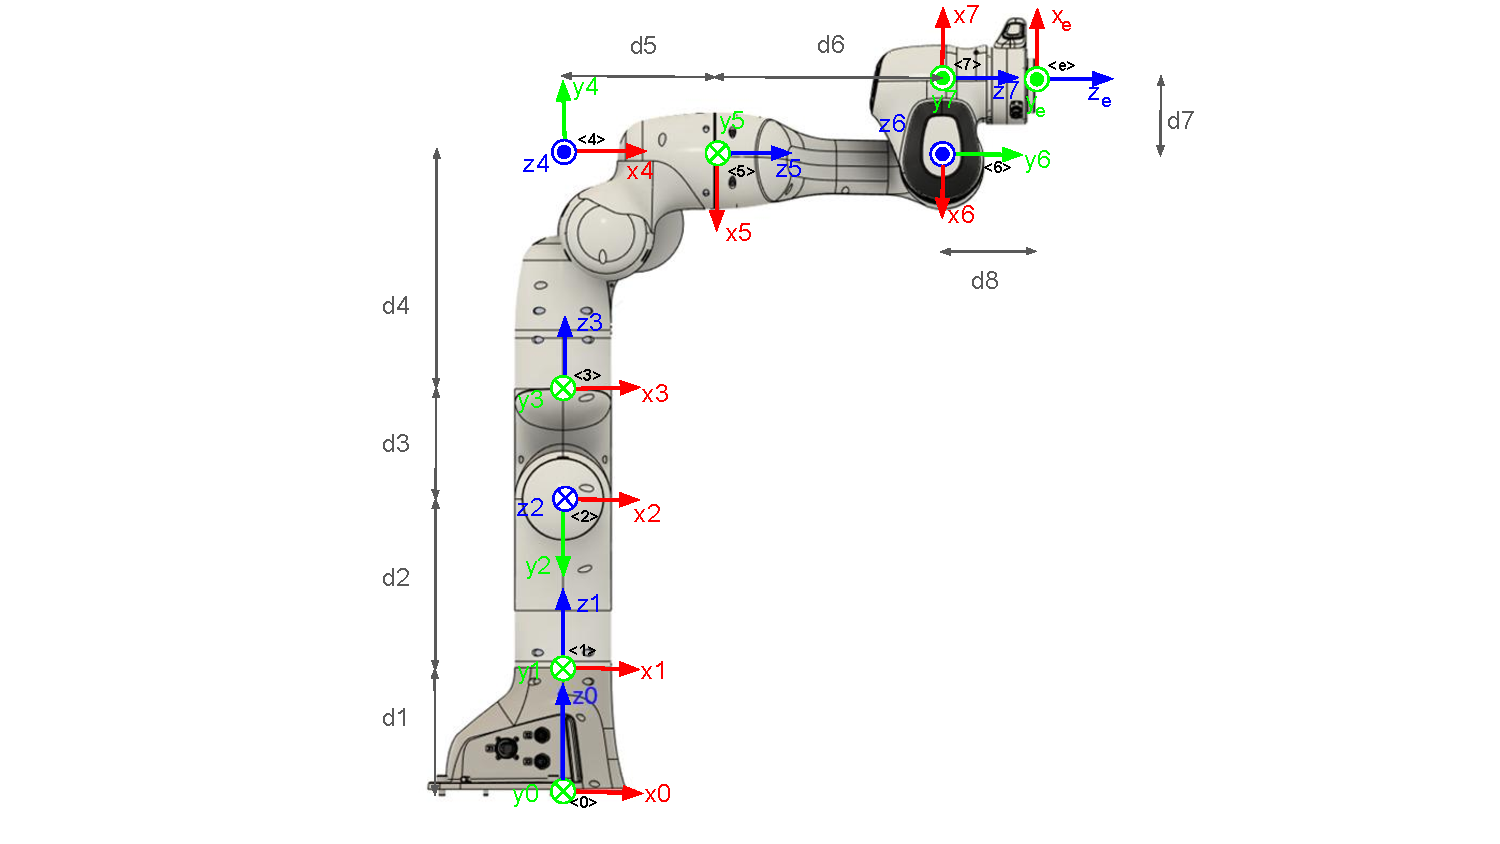
\includegraphics[width=1\linewidth]{Resources/franka.pdf}
\caption{exercise 5 frames}
\label{fig:ex2}
\end{figure}

Figure \ref{fig:ex2} shows the frame tree for the 7 joints of the Franka robot. With reference to the figure, use the geometric definition of the transformation matrix to compute by hand the following matrices.
\begin{itemize}
\item \textbf{Q5.1} \hspace{10mm} $^0_1 T$
\item \textbf{Q5.2} \hspace{10mm} $^1_2 T$
\item \textbf{Q5.3} \hspace{10mm} $^2_3 T$
\item \textbf{Q5.4} \hspace{10mm} $^3_4 T$
\item \textbf{Q5.5} \hspace{10mm} $^4_5 T$
\item \textbf{Q5.6} \hspace{10mm} $^5_6 T$
\item \textbf{Q5.7} \hspace{10mm} $^6_7 T$
\item \textbf{Q5.8} \hspace{10mm} $^7_e T$
\end{itemize}

You \textbf{MUST} compute the matrices \textbf{WITHOUT} using mathematical software.

\newpage
\section{Solution} \label{P1}
% Write some intro

The second assignment of Modelling and Control of Manipulators focuses on manipulators’ geometry and
direct kinematics. The aim of the lab is given a CAD model of an industrial 7 DoF manipulator give the initial transformation matrix, then implement in Matlab a method to compute the geometric model and the transformation matrices from the base to each joint. Finally, we have to implement a function which given the geometric model, the joint types and the number of joints can compute the Jacobian matrix of a generic serial manipulator.

\subsection{Q1.1}

For the first question, we have to complete the Matlab function \textit{BuildTree}  based on the CAD model of the industrial 7 DoF manipulator \ref{fig:ex2}. The robot is in a singular configuration, and we can easily compute each transformation matrix between each frame. 

We will use the general formula of the transformation matrix between two frames
\[
^{i-1}_i T = \begin{pmatrix}
        ^{i-1}_i R & ^{i-1}O_i & \\
        \textbf{0} & 1 & \\
        \end{pmatrix}
\]

For the transformation matrix from the base frame to frame 1, we only have a translation along the z-axis of 0.105 m without rotation. So, the transformation matrix is as follows:

\[^b_1 T = \begin{pmatrix}
        1 & 0 & 0 & 0 \\
        0 & 1 & 0 & 0 \\
        0 & 0 & 1 & 0.105 \\
        0 & 0 & 0 & 1 \\
    \end{pmatrix}\]
\\
For the transformation matrix from frame 1 to frame 2, we have a translation along the z-axis of 0.110 m. And a vector (x,y,z) is transformed into a vector (y,z,x) from frame 1 to frame 2. So, the transformation matrix is as follows:

\[^1_2 T = \begin{pmatrix}
        0 & 1 & 0 & 0 \\
        0 & 0 & 1 & 0 \\
        1 & 0 & 0 & 0.110 \\
        0 & 0 & 0 & 1 \\
    \end{pmatrix}\]
\\
For the transformation matrix from frame 2 to frame 3, we have a translation along the x-axis of 0.1 m. In addition, a vector (x, y, z) is transformed to a vector (z,-y,x). So, the transformation matrix is as follows:

\[^2_3 T = \begin{pmatrix}
        0 & 0 & 1 & 0.1 \\
        0 & -1 & 0 & 0 \\
        1 & 0 & 0 & 0 \\
        0 & 0 & 0 & 1 
    \end{pmatrix}\]

For the transformation matrix from frame 3 to frame 4, we have a translation along the z-axis of 0.325 m. Then, a vector (x,y,z) is transformed to a vector (z,-y,x). So, the transformation matrix is as follows: 

\[^3_4 T = \begin{pmatrix}
        0 & 0 & 1 & 0 \\
        0 & -1 & 0 & 0 \\
        1 & 0 & 0 & 0.325 \\
        0 & 0 & 0 & 1 
    \end{pmatrix}\]

For the transformation matrix from frame 4 to frame 5, we have a translation along the x-axis of 0.095 m. Then, a vector (x,y,z) is transformed to a vector (-y,-z,x). So, the transformation matrix is as follows : 

\[^4_5 T = \begin{pmatrix}
        0 & 0 & 1 & 0.095 \\
        -1 & 0 & 0 & 0 \\
        0 & -1 & 0 & 0 \\
        0 & 0 & 0 & 1 
    \end{pmatrix}\]

For the transformation matrix from frame 5 to frame 6, we have a translation along the z-axis of 0.095 m. Then, a vector (x,y,z) is transformed to a vector (-x,-y,z). So, the transformation matrix is as follows: 

\[^5_6 T = \begin{pmatrix}
        -1 & 0 & 0 & 0 \\
        0 & -1 & 0 & 0 \\
        0 & 0 & 1 & 0.095 \\
        0 & 0 & 0 & 1 
    \end{pmatrix}\]
    
For the transformation matrix from frame 6 to frame e of the end effector, we have a translation along the z-axis of 0.355 m and no rotation. So, the transformation matrix is as follows: 

\[^6_e T = \begin{pmatrix}
        1 & 0 & 0 & 0 \\
        0 & 1 & 0 & 0 \\
        0 & 0 & 1 & 0.355 \\
        0 & 0 & 0 & 1 \\
    \end{pmatrix}\]

Now, we can fill the \textit{BuildTree} function with these matrices.

\newpage
\subsection{Q1.2}

Here, we need to build the method called $updateDirectGeometry$ of the $geometricModel$ class which should compute the model matrices as a function of the joint position $q$. Each joint contributes to the robot's motion by either rotating (revolute joint) or translating (prismatic joint). To model these motions mathematically, we compute a transformation matrix for each joint. Here's how it's done:

\subsubsection{Revolute Joints}  

A revolute joint rotates around its local z-axis. The transformation matrix that represents this rotation is given by:

\[
T_z(\theta_i) = 
\begin{pmatrix}
\cos(q_i) & -\sin(q_i) & 0 & 0 \\
\sin(q_i) & \cos(q_i) & 0 & 0 \\
0 & 0 & 1 & 0 \\
0 & 0 & 0 & 1 \\
\end{pmatrix}
\]

Here, \( q_i=\theta_i \) is the current angle of rotation for the joint i.

\subsubsection{Prismatic Joints}

A prismatic joint translates along its local z-axis. The transformation matrix for this translation is:

\[
T_z(d_i) =
\begin{pmatrix}
1 & 0 & 0 & 0 \\
0 & 1 & 0 & 0 \\
0 & 0 & 1 & q_i \\
0 & 0 & 0 & 1 \\
\end{pmatrix}
\]

Here, \( q_i = d_i \) represents the value of the translation along the z-axis in meter.

\subsubsection{Input}

We will apply this method with the vector $q$ below : 
\[
q = \begin{pmatrix}
    \frac{\pi}{4} & -\frac{\pi}{4} & 0 & -\frac{\pi}{4} & 0 & 0.15 & \frac{\pi}{4}
\end{pmatrix}
\]

And the with this joint type vector corresponding to the robot:

\[
jointType = \begin{pmatrix}
    0 & 0& 0&0 &0&1 &0
\end{pmatrix}
\]

\subsubsection{Results}

\paragraph{Joint 1 : revolute joint} 
\subparagraph{We substitute with $\theta_1 = \frac{\pi}{4}$ in $T_z(\theta)$. The result is shown below after performing a product between $^{b}_1T$ and $T_z(\theta)$. For revolute joints, the translation vector is not affected by this operation.}

\[
\begin{pmatrix}
1 & 0 & 0 & 0 \\
0 & 1 & 0 & 0 \\
0 & 0 & 1 & 0.105 \\
0 & 0 & 0 & 1 \\
\end{pmatrix}
\
\begin{pmatrix}
0.7071 & -0.7071 & 0 & 0 \\
0.7071 & 0.7071 & 0 & 0 \\
0 & 0 & 1 & 0 \\
0 & 0 & 0 & 1 \\
\end{pmatrix}
=
\begin{pmatrix}
0.7071 & -0.7071 & 0 & 0 \\
0.7071 & 0.7071 & 0 & 0 \\
0 & 0 & 1 & 0.105 \\
0 & 0 & 0 & 1 \\
\end{pmatrix}
\]

\paragraph{Joint 2 : revolute joint}
\subparagraph{We substitute with $\theta_2 = -\frac{\pi}{4}$ in $T_z(\theta)$. The result is shown below after performing a product between $^{1}_2T$ and $T_z(\theta)$. For revolute joints, the translation vector is not affected by this operation.}
\[
\begin{pmatrix}
0 & 1 & 0 & 0 \\
0 & 0 & 1 & 0 \\
1 & 0 & 0 & 0.110 \\
0 & 0 & 0 & 1 \\
\end{pmatrix}
\
\begin{pmatrix}
0.7071 & 0.7071 & 0 & 0 \\
-0.7071 & 0.7071 & 0 & 0 \\
0 & 0 & 1 & 0 \\
0 & 0 & 0 & 1 \\
\end{pmatrix}
=
\begin{pmatrix}
-0.7071 & 0.7071 & 0 & 0 \\
0 & 0 & 1 & 0 \\
0.7071 & 0.7071 & 0 & 0.110 \\
0 & 0 & 0 & 1 \\
\end{pmatrix}
\]

\paragraph{Joint 3 : revolute joint}
\subparagraph{We substitute with $\theta_3 = 0$ in $T_z(\theta)$. The result is shown below after performing a product between $^{2}_3T$ and $T_z(\theta)$. The rotation matrix in this case is the identity matrix, indicating that no changes are applied to \( ^{2}_3T \) overall.}
\[
\begin{pmatrix}
0 & 0 & 1 & 0.100 \\
0 & -1 & 0 & 0 \\
1 & 0 & 0 & 0 \\
0 & 0 & 0 & 1 \\
\end{pmatrix}
\
\begin{pmatrix}
1 & 0 & 0 & 0 \\
0 & 1 & 0 & 0 \\
0 & 0 & 1 & 0 \\
0 & 0 & 0 & 1 \\
\end{pmatrix}
=
\begin{pmatrix}
0 & 0 & 1 & 0.100 \\
0 & -1 & 0 & 0 \\
1 & 0 & 0 & 0 \\
0 & 0 & 0 & 1 \\
\end{pmatrix}
\]

\paragraph{Joint 4 : revolute joint}
\subparagraph{We substitute with $\theta_4 = -\frac{\pi}{4}$ in $T_z(\theta)$. The result is shown below after performing a product between $^{3}_4T$ and $T_z(\theta)$. For revolute joints, the translation vector is not affected by this operation.}
\[
\begin{pmatrix}
0 & 0 & 1 & 0 \\
0 & -1 & 0 & 0 \\
1 & 0 & 0 & 0.325 \\
0 & 0 & 0 & 1 \\
\end{pmatrix}
\
\begin{pmatrix}
0.7071 & 0.7071 & 0 & 0 \\
-0.7071 & 0.7071 & 0 & 0 \\
0 & 0 & 1 & 0 \\
0 & 0 & 0 & 1 \\
\end{pmatrix}
=
\begin{pmatrix}
0 & 0 & 1 & 0 \\
0.7071 & -0.7071 & 0 & 0 \\
0.7071 & 0.7071 & 0 & 0.325 \\
0 & 0 & 0 & 1 \\
\end{pmatrix}
\]

\paragraph{Joint 5 : revolute joint}
\subparagraph{We substitute with $\theta_5 = 0$ in $T_z(\theta)$. The result is shown below after performing a product between $^{4}_5T$ and $T_z(\theta)$. The rotation matrix in this case is the identity matrix, indicating that no changes are applied to \( ^{4}_5T \) overall.}
\[
\begin{pmatrix}
0 & 0 & 1 & 0.095 \\
-1 & 0 & 0 & 0 \\
0 & -1 & 0 & 0 \\
0 & 0 & 0 & 1 \\
\end{pmatrix}
\
\begin{pmatrix}
1 & 0 & 0 & 0 \\
0 & 1 & 0 & 0 \\
0 & 0 & 1 & 0 \\
0 & 0 & 0 & 1 \\
\end{pmatrix}
=
\begin{pmatrix}
0 & 0 & 1 & 0.095 \\
-1 & 0 & 0 & 0 \\
0 & -1 & 0 & 0 \\
0 & 0 & 0 & 1 \\
\end{pmatrix}
\]

\paragraph{Joint 6 : primastic joint}
\subparagraph{We substitute with $d_6 = 0.15$ m in $T_z(d_6)$. The result is shown below after performing a product between $^{6}_7T$ and $T_z(d_6)$. For prismatic joints, the rotation matrix is not affected by this operation and we can see the translation vector in the output has a change in k direction, which is basically the sum of the values 0.095 and 0.150.}

\[
\begin{pmatrix}
-1 & 0 & 0 & 0 \\
0 & -1 & 0 & 0 \\
0 & 0 & 1 & 0.095 \\
0 & 0 & 0 & 1 \\
\end{pmatrix}
\
\begin{pmatrix}
1 & 0 & 0 & 0 \\
0 & 1 & 0 & 0 \\
0 & 0 & 1 & 0.150 \\
0 & 0 & 0 & 1 \\
\end{pmatrix}
=
\begin{pmatrix}
-1 & 0 & 0 & 0 \\
0 & -1 & 0 & 0 \\
0 & 0 & 1 & 0.245 \\
0 & 0 & 0 & 1 \\
\end{pmatrix}
\]

\paragraph{Joint 7 : revolute joint}
\subparagraph{We substitute with $\theta_7 = \frac{\pi}{4}$ in $T_z(\theta)$. The result is shown below after performing a product between $^{5}_6T$ and $T_z(\theta)$. For revolute joints, the translation vector is not affected by this operation.}
\[
\begin{pmatrix}
1 & 0 & 0 & 0 \\
0 & 1 & 0 & 0 \\
0 & 0 & 1 & 0.355 \\
0 & 0 & 0 & 1 \\
\end{pmatrix}
\
\begin{pmatrix}
0.7071 & -0.7071 & 0 & 0 \\
0.7071 & 0.7071 & 0 & 0 \\
0 & 0 & 1 & 0 \\
0 & 0 & 0 & 1 \\
\end{pmatrix}
=
\begin{pmatrix}
0.7071 & -0.7071 & 0 & 0 \\
0.7071 & 0.7071 & 0 & 0 \\
0 & 0 & 1 & 0.355 \\
0 & 0 & 0 & 1 \\
\end{pmatrix}
\]

\paragraph{Remark}
\subparagraph{For each joint, we find the same transformation matrices as the Matlab output of the function $geometricModel$.}

\newpage

\subsection{Q1.3}

\subsubsection{Method}
For this question, we have to implement the method of geometricModel called $getTransformWrtBase()$ which should compute the transformation matrix from the base to a given frame named $k$. The function will first check if $k$ is more than 0 and lower than the number of joint of the robot. Then, starting from the identity matrix (corresponding to  $^{b}_{b} T$) , it will loop with i from 1 to k by doing a right product on the previous matrix with the transformation matrix $^{i-1}_{i} T$. Indeed, we have that $^b_k T = {^b_1 T} {^1_2 T} ...  {^{k-1}_k T} $.

\subsubsection{Compute $^b_e T$}

To compute $^b_e T$, we have to use the function $getTransformWrtBase$ just written with the total number of joints as argument. We can have that number by computing the length of the $jointType$ list. Then, the function will compute the transformation matrix from the base frame to the end effector by doing this calculus : $^b_e T = {^b_1 T} {^1_2 T} {^2_3 T} {^3_4 T} {^4_5 T} {^5_6 T} {^6_e T} $ . 

Finally, with \[
q = \begin{pmatrix}
    \frac{\pi}{4} & -\frac{\pi}{4} & 0 & -\frac{\pi}{4} & 0 & 0.15 & \frac{\pi}{4}
\end{pmatrix}
\] we obtain : 

\[^b_e T(q) = \begin{pmatrix}
        -0.5 & -0.5 & -0.7071 & -0.7039 \\
        0.5 & 0.5 & -0.7071 & -0.7039 \\
        0.7071 & -0.7071 & 0 & 0.5155 \\
        0 & 0 & 0 & 1 \\
    \end{pmatrix}\]

In this matrix, we can see that the orientation of the end effector is rotated around the three axis of the base frame and its position with respect of the base frame is $(x_e,y_e,z_e)=(-0.7039, -0.7039, 0.5155)$.

\subsubsection{Compute $^5_3 T$}

To compute $^5_3 T$, we have to do some calculation. 
First, let's compute $^3_5 T$

\[ ^3_5 T = {^3_b T}  {^b_5 T} = {^b_3 T}^{-1} {^b_5 T}  \]

Then, 

\[ ^5_3 T = {^3_5 T}^{-1} = {({^b_3 T}^{-1} {^b_5 T})}^{-1} \]

And we know that we can get $^b_3 T$ with $getTransformWrtBase(3)$ and $^b_5 T$ with $getTransformWrtBase(5)$. So, we can compute $^5_3 T$ in Matlab with \[
q = \begin{pmatrix}
    \frac{\pi}{4} & -\frac{\pi}{4} & 0 & -\frac{\pi}{4} & 0 & 0.15 & \frac{\pi}{4}
\end{pmatrix}
\] and we obtain :

\[^5_3 T(q) = \begin{pmatrix}
        0 & 0.7071 & -0.7071 & -0.2298 \\
        -1 & 0 & 0 & 0 \\
        0 & 0.7071 & 0.7071 & -0.3248 \\
        0 & 0 & 0 & 1 \\
    \end{pmatrix}\]


In this matrix, we can notice that $\frac{\sqrt{2}}{2} \approx 0.7071$. Moreover, we know that $sin(\frac{\pi}{4}) = \frac{\sqrt{2}}{2} $ and $cos(\frac{\pi}{4}) = \frac{\sqrt{2}}{2} $. So it's coherent with the rotation of $\frac{\pi}{4}$ due to $q_4$ as $q_3=0$ and $q_5=0$.

Finally, we find the same result as computing directly ${({^3_4 T(0)} {^4_5 T(\frac{\pi}{4})})}^{-1}$ using the Q1.2.

\newpage
\subsection{Q1.4}
\subparagraph{Here, we need to build the method called $updateJacobian$ of the $kinematicModel$ class. As we can have the transformation matrix from the base to a given frame, we can compute the Jacobian matrix of the manipulator for the end-effector like below. So, we need to find the angular and linear parts of the Jacobian for either revolute and prismatic joints.  }


\[\mathbf{^0 J_{e/b}} = \begin{pmatrix}
        \mathbf{^0 J^A_{1}} & \mathbf{^0 J^A_{2}} &  ... & \mathbf{^0 J^A_{e}} \\
        \mathbf{^0 J^L_{e/1}} & \mathbf{^0 J^L_{e/2}} & ... & \mathbf{^0 J^L_{e/e}} \\
    \end{pmatrix}\]

\subsubsection{Angular Jacobian} 
\subparagraph{The Angular Jacobian for any revolute joint is the third column of the rotation matrix of the joint with respect to the base $^0\mathbf{K_i}$. On the other hand, for prismatic joints, it's a zero vector since there's no any angular velocity that can be generated from translation. So, we have : }
\[
^{0}\mathbf{J}{}^A_i = 
\begin{cases} 
^{0}\mathbf{K}_i & \text{if } \Gamma_i = R \\ 
\mathbf{0} & \text{if } \Gamma_i = P 
\end{cases}
\]

\subsubsection{Linear Jacobian} 
\subparagraph{The Linear Jacobian for any revolute joint is the cross product between $^0\mathbf{K_i}$ and, $\mathbf{r}_{e/i} = \mathbf{r}_{e} - \mathbf{r}_{i} $ which are:
\newline
$^0\mathbf{K_i}$ : the third column of the rotation matrix of the joint i with respect to the base.
\newline
$\mathbf{r}_{e}$ : a vector that represents the position of the end effector, with respect to base.
\newline
$\mathbf{r}_{i}$ : a vector that represents the position of the joint i with respect to base.
\newline
On the other hand, for prismatic joints, it's just $^0\mathbf{K_i}$. So we have : }
\[
{}^{0}\mathbf{J}{}^L_{e/i} = 
\begin{cases} 
\left( ^0\mathbf{K}_i \times (\mathbf{r}_{e} - \mathbf{r}_{i})  \right) & \text{if } \Gamma_i = R \\ 
^0\mathbf{K}_i & \text{if } \Gamma_i = P
\end{cases}
\]
\subsubsection{Initial Configuration}
\subparagraph{These are the initial joint parameters :}
\[
q_{init} = \begin{pmatrix}
    \frac{\pi}{4} & -\frac{\pi}{4} & 0 & -\frac{\pi}{4} & 0 & 0.15 & \frac{\pi}{4}
\end{pmatrix}
\]
\subparagraph{In the figures \ref{fig:Initial Configuration1} and \ref{fig:Initial Configuration2}, we can see the initial configuration of the robot with respect to the base frame. All joint positions are marked with circles.}

\begin{figure}[h!]
    \begin{minipage}{0.5\textwidth}
        \centering
        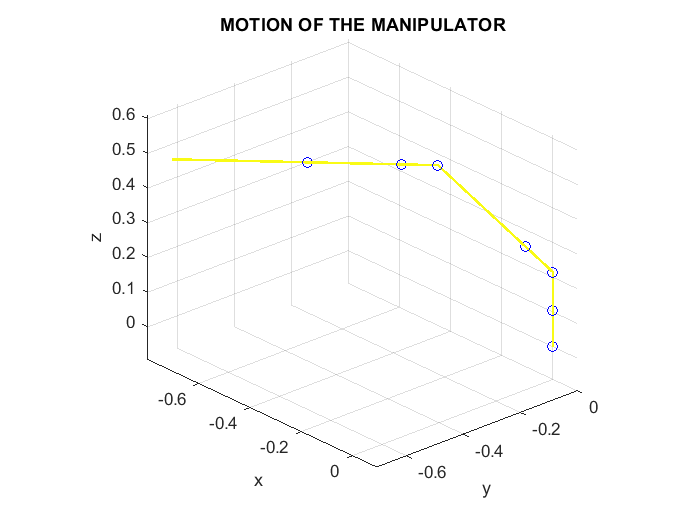
\includegraphics[width=\linewidth]{template_MCM_lab2_2024_25/Resources/q1.1.png}
        \caption{Isometric View of the Initial Configuration}
        \label{fig:Initial Configuration1}
    \end{minipage}%
    \hfill
    \begin{minipage}{0.5\textwidth}
        \centering
        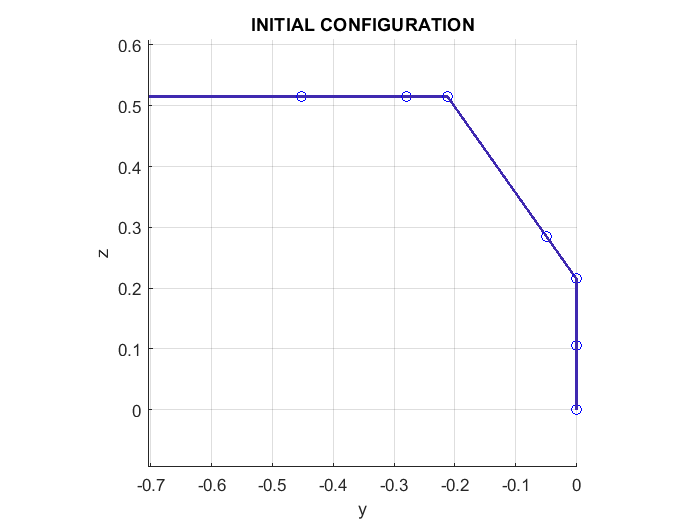
\includegraphics[width=\linewidth]{template_MCM_lab2_2024_25/Resources/q1.3.png}
        \caption{Side View of the Initial Configuration}
        \label{fig:Initial Configuration2}
    \end{minipage}
\end{figure}

\subsubsection{Final Configurations}
\subparagraph{These are the final joint parameters :}
\[
q_f = \begin{pmatrix}
    \frac{\pi}{4} + \frac{\pi}{6} & -\frac{\pi}{4} & 0 & -\frac{\pi}{4} & 0 & 0.15 & \frac{\pi}{4}
\end{pmatrix}
\]
\subparagraph{The robot transitions to a new configuration where the first joint has to rotate of $\pi/6$ around the $z_0$ axis. The remaining joints don't have rotations or translations from their initial configuration. So the motion of the robot is circular around the $z_0$ axis as we can see in the figure \ref{fig:Final Configuration1} in order to arrive in the final configuration as we can see in figure \ref{fig:Final Configuration2}}

\begin{figure}[h!]
    \begin{minipage}{0.5\textwidth}
        \centering
        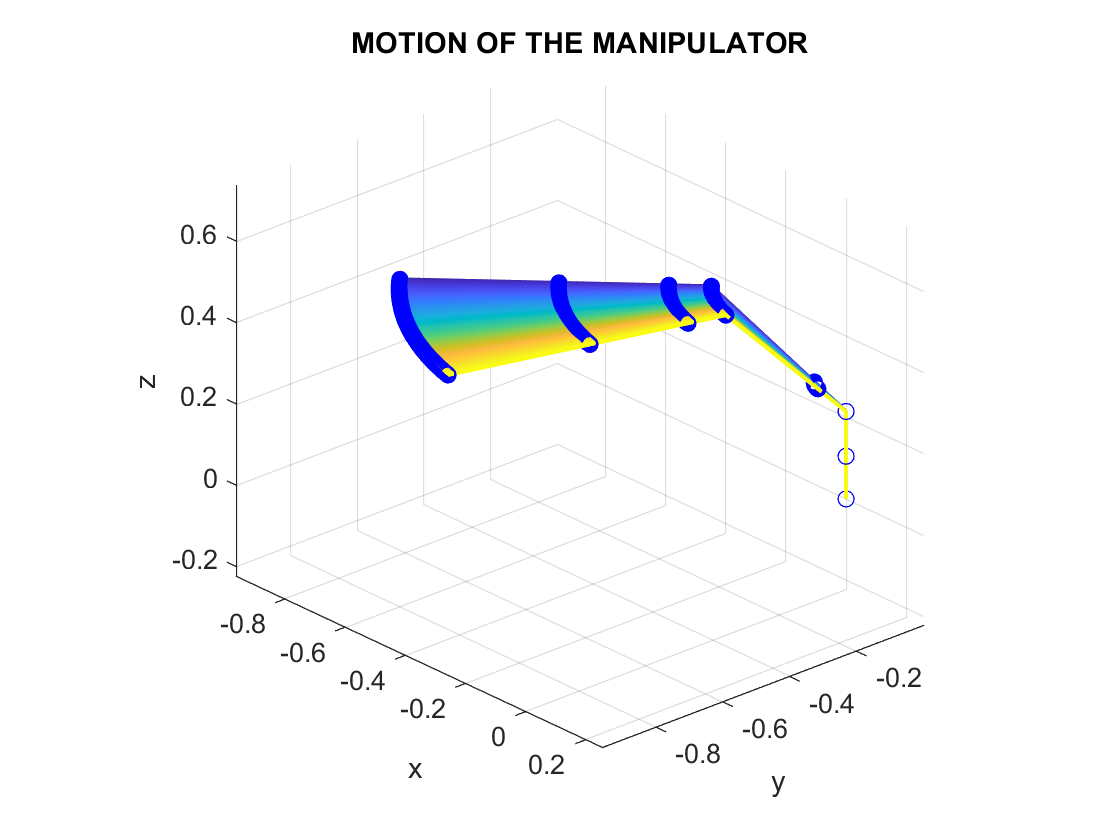
\includegraphics[width=\linewidth]{template_MCM_lab2_2024_25/Resources/motion_of_the_manipulator.png}
        \caption{Isometric View of the Final Configuration}
        \label{fig:Final Configuration1}
    \end{minipage}%
    \hfill
    \begin{minipage}{0.5\textwidth}
        \centering
        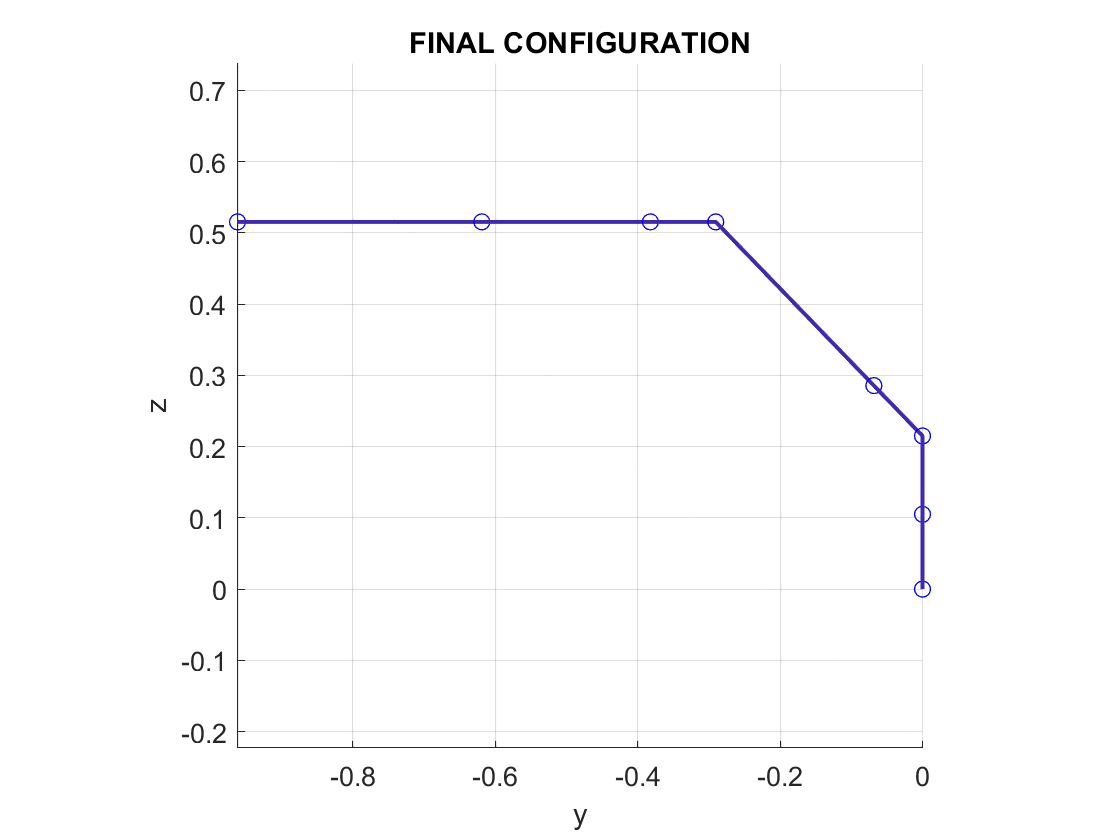
\includegraphics[width=\linewidth]{template_MCM_lab2_2024_25/Resources/final_configuration.png}
        \caption{Side View of the Final Configuration}
        \label{fig:Final Configuration2}
    \end{minipage}
\end{figure}

\subsubsection{Jacobian}
\subparagraph{
The Jacobian matrix, J(q) gives the relationship between joint velocities and the end-effector's linear and angular velocities. The Matlab function $kinematicModel$ gives us this Jacobian matrix for the robot with $q_{init}$ :
}

\[J(q_{init}) = \begin{pmatrix}
        0 & -0.7071 & -0.5 & -0.7071 & -0.7071 & 0 & -0.7071 \\
        0 & 0.7071 & -0.5 & 0.7071 & -0.7071 & 0 & -0.7071 \\
        1 & 0 & 0.7071 & 0 & 0 & 0 & 0 &  \\
        0.7039 & 0.2125 & 0.3475 & 0 & 0 & -0.7071 & 0 \\
        -0.7039 & 0.2125 & -0.3475 & 0 & 0 & -0.7071 & 0 \\
        0 & 0.9955 & 0 & 0.6950 & 0 & 0 & 0 \\
    \end{pmatrix}\]

% TODO : Comment the rank and the result, can be commandable because Xp = J q

\subparagraph{The Jacobian matrix is rank 6, indicating 6 linearly independent rows or columns. This suggests the manipulator has 6 degrees of freedom (DOF) in its task space, allowing full control over the end-effector's linear and angular velocities. Since the matrix has more columns than rows, there may be one redundant degree of freedom, possibly due to passive or redundant joints. With this Jacobian matrix $J(q_{init})$, we could compute the end-effector's linear and angular velocities near the initial state.}

% Add bTe of the final pose ? 





\section{Exercise 2} \label{P2}

\textit{[Comment] Same structure of exercise 1 } 
\section{Exercise 3} \label{P3}

\textit{[Comment] Same structure of exercise 1 } 

\section{Exercise 4} \label{P4}

\textit{[Comment] Same structure of exercise 1 } 

\section{Exercise 5} \label{P5}
\subsection{Q5.1}
$^0_1 T = \begin{pmatrix}
        ? & ? & ? & ? \\
        ? & ? & ? & ? \\
        ? & ? & ? & ? \\
        ? & ? & ? & ?
    \end{pmatrix}$
    
\textit{[Comment] Same structure for the other matrices } 


\pagebreak

\section{Appendix}
\textit{[Comment] Add here additional material (if needed)} 
\subsection{Appendix A}

\subsection{Appendix B}


\end{document}
